\chapter{Sistema Multiagentes e Regras de Inferência}
\label{sec:SistMult}

Neste capítulo, será feita uma breve descrição de Sistemas MultiAgentes. Na Seção \ref{sec:Agent}, falaremos sobre Agentes. A Seção \ref{sec:SMA} detalha conceitos de Sistemas MultiAgentes. A Seção \ref{sec:FerramentaSMA} descreve ferramentas analisadas nesse trabalho. Por fim, na Seção, \ref{sec:RegraInfer}, serão mostrados motores de inferência para raciocínio automático utilizado nesse trabalho.

\subsection{Agentes} \label{sec:Agent}

\begin{figure}[htb!]
\centering
%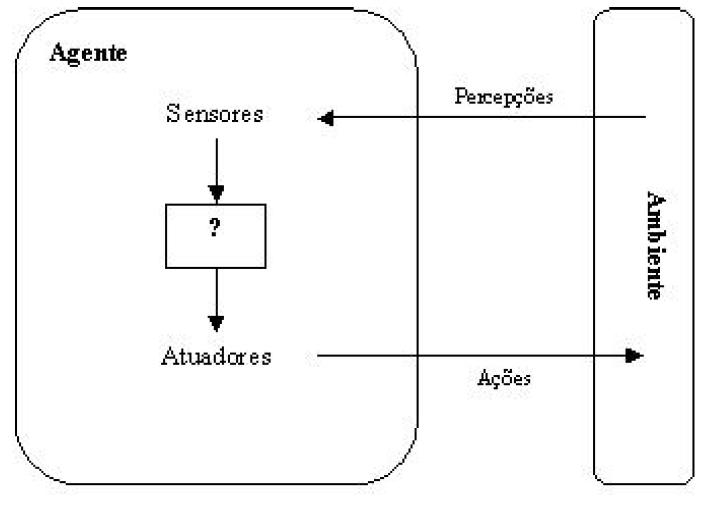
\includegraphics[angle=0,width=0.6\textwidth]{imagens//agentes.JPG}
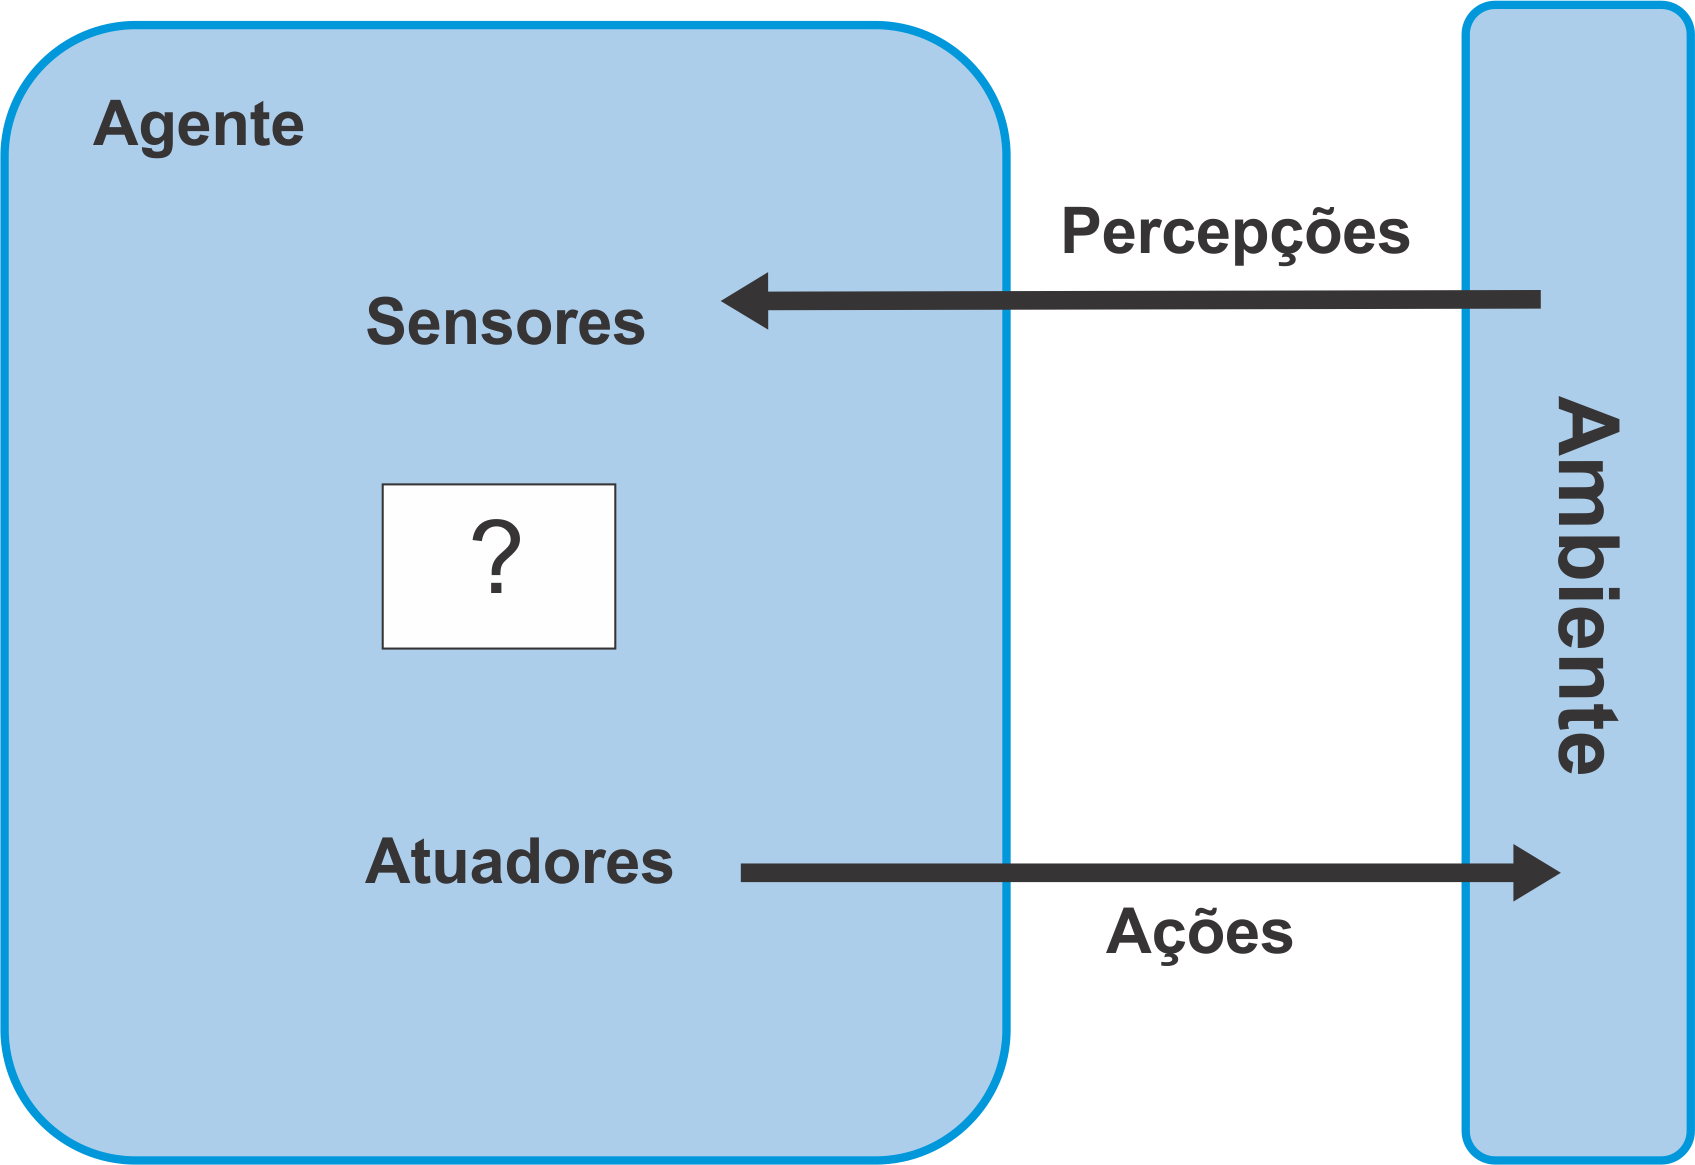
\includegraphics[angle=0,width=0.6\textwidth]{imagens//Agentes1sem.png}
\caption{Arquitetura de um agente inteligente (Adaptado de~\citep{Russell:2002}).} \label{fig:Agente}
\end{figure}


Um agente~\citep{Russell:2002} é uma entidade capaz de perceber seu ambiente através de sensores e de agir sobre esse ambiente através de atuadores Figura~\ref{fig:Agente}. Cada agente exibe duas características fundamentais: é capaz de agir de forma autônoma tomando decisões que levam à satisfação dos seus objetivos; e é capaz de interagir com outros agentes utilizando protocolos de interação social inspirados nos humanos e incluindo pelo menos algumas das seguintes funcionalidades - coordenação, cooperação, competição e negociação~\citep{Russell:2002}.

\subsection{SMAs} \label{sec:SMA}

\begin{figure}[htb!]
\centering
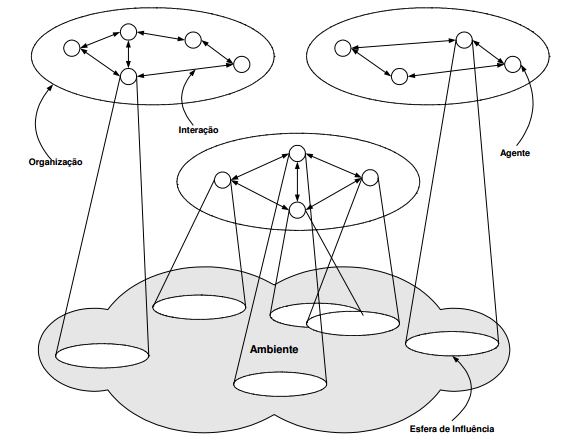
\includegraphics[angle=0,width=0.7\textwidth]{imagens//multiAgent.png}
\caption{Estrutura de um Sistema Multi-Agente (Adaptado de~\citep{wooldridge2009introduction:2009}).} \label{fig:MultiAgent}
\end{figure}

Os Sistemas MultiAgente (SMAs) incluem diversos agentes que interagem ou trabalham em
conjunto, podendo compreender agentes homogêneos ou heterogêneos. Cada agente opera
assincronamente com respeito aos outros agentes~\citep{wooldridge2009introduction:2009}. Para que um agente possa operar como parte do sistema, é necessária a existência de uma infraestrutura que permita a
comunicação e/ou interação entre os agentes que compõem o SMA Figura~\ref{fig:MultiAgent}.

\subsection{Ferramentas para SMAs} \label{sec:FerramentaSMA}

Nesta seção, inicialmente descreveremos ferramentas para a construção de SMAs e em seguida faremos uma comparação entre elas.

\subsubsection{Descrição das Ferramentas}

\subsubsection*{Breve}

É uma ferramenta livre, que permite uma criação de sistemas multiagentes 3D. Ela utiliza como linguagem de programação o Python, ou uma linguagem de \textit{script} com o nome de Steve, ela permite definir comportamentos dos agentes em um mundo 3D e observar como eles interagem. 

\subsubsection*{Cormas}

É uma ferramenta livre, um framework de simulação baseado em agentes. Ela utiliza como linguagem de programação o Visual Works, que permite desenvolver para o SmallTalk, sendo orientada a objeto.   

\subsubsection*{JADE}

O JADE (\textit{Java Agent DEvelopment Framework})~\citep{Bellifemine:2003} segue os padrões da FIPA (Foundation for Intelligent Physical Agents),  uma organização responsável por especificar padrões para o desenvolvimento de tecnologias baseadas em agentes inteligentes. O JADE possibilita e facilita a programação de agentes inteligentes usando Java, possui muitos atributos e características que a tornam ideal para a implementação de agentes, além de simplificar o desenvolvimento por disponibilizar um \textit{framework} que trata a comunicação, o ciclo de vida do agente e o monitoramento da execução, entre outras.

\subsubsection*{Jadex}

É um pacote construído para permitir o desenvolvimento de agentes de acordo com a FIPA e a arquitetura BDI de agentes. JADEX permite a construção de agentes de software seguindo os conceitos do modelo BDI (Belief Desire Intention);

\begin{itemize}
\item [i)] Usa tecnologias como XML e Java;
\item [ii)] JADEX é projetado para facilitar a implementação de agentes em Java, e, portanto permite o reuso de várias ferramentas e bibliotecas.
\end{itemize}
	Um agente JADEX é também um agente JADE e, portanto todas as ferramentas disponíveis em JADE podem ser usadas também para desenvolver agentes em JADEX. A maior parte da plataforma JADE lida com a visão externa de um agente, que não difere entre um agente JADE ou JADEX.

\subsubsection*{Zeus}

É um ambiente integrado para a construção rápida de aplicações com agentes colaborativos. A documentação da ferramenta Zeus é abundante, e coloca uma forte ênfase na importância da metodologia aspecto de Zeus ("A metodologia de criação do agente é vital para o uso do Zeus"). A metodologia de Zeus usa a decomposição de quatro estágios para o mesmo desenvolvimento de agente como em nossa análise, respectivamente análise de domínio, design, realização e apoio a execução.

\subsubsection*{JAS} 

É uma ferramenta em Java para a simulação de agentes. Possui um mecanismo de tempo para eventos discretos, com sondas estáticas embutidas, redes neurais e algoritmos genéticos.

 
\subsubsection*{MADKIT}

É uma ferramenta livre modular e uma plataforma escalave para multiagetens. Ferramenta que trabalha com Java e foi escrito em Java.   

 
\subsubsection*{JASON}

É uma maneira rápida de eventos discretos multiagentes que tem um núcleo com biblioteca de simulação em Java, projetado para ser a base para grandes simulações personalizadas, e também para fornecer mais funcionalidade com suficiência para simulação. MASON contém uma biblioteca de modelo e um conjunto opcional de ferramentas de visualização em 2D e 3D.

\subsubsection*{MicrosoftAgent}

É um conjunto de serviços programável por software que suporta a apresentação dos personagens animados interativos. Os desenvolvedores podem usar personagens como assistentes interativos para apresentar, orientar, entreter, ou melhorar as suas páginas Web ou aplicações além do uso convencional de janelas, menus e controles.

\subsubsection*{NetLogo}

É um ambiente de multi-agente livre com modelagem programável. Ele é usado por dezenas de milhares de estudantes, professores e pesquisadores do mundo todo. É de autoria de Uri Wilensky e desenvolvido no CCL.  


\subsubsection*{Open Architecture Agent (OAA)}

É uma ferramenta focada na construção de comunidades distribuídas de agentes, onde o agente é definido como qualquer processo de software que atenda as convenções da sociedade OAA. Um agente satisfaz este requisito, registrando os serviços que ela pode fornecer em uma forma aceitável, por ser capaz de falar a linguagem de comunicação interagente (ICL), e através da partilha de funcionalidades comuns a todos os agentes OAA. 

\subsubsection*{AgentBuilder}

É um conjunto de ferramentas integradas para a construção de software de agentes inteligentes. É desenvolvido pela Reticular Systems Inc., e está fundamentada no modelo de Agents BDI. Esta ferramenta é notável tanto pela alta qualidade dos seu software e do modelo conhecido.


\subsubsection*{Shell for Simulated Agent Systems (SeSAM)} 

SESAM (Shell para Sistemas de Agente simulado)~\citep{Sesam:2011} fornece um ambiente genérico para modelagem e experimentação de agente baseado em simulação. Está especialmente voltada ao fornecimento de uma ferramenta para a construção fácil de modelos complexos, que incluem interdependências dinâmica ou comportamento emergente. 

\subsubsection*{SIM Agent}

É uma ferramenta com uma gama de recursos para pesquisa e ensino relacionadas com o desenvolvimento de agentes que interagem em ambientes de diferentes graus e tipos de complexidade. Pode ser executado como uma ferramenta de simulação pura. Ela foi originalmente desenvolvida para suportar uma pesquisa exploratória sobre humano, como agentes inteligentes, mas também tem sido usado para projetos de estudantes a desenvolver uma variedade de jogos e simulações interativas.

\subsubsection*{Simulation of Cognitive Agents (SimCog)}

É uma plataforma genérica para SMA de simulação baseada em agentes cognitivos. Ele começou em 2001, no Departamento de Informática da Universidade de Lisboa.

\subsubsection*{StartLogo}

É um ambiente de modelagem programável para explorar o funcionamento de sistemas descentralizados. Sistemas que são organizados sem um gerente, coordenado sem um gerenciador. Com StarLogo, você pode modelar, muitos fenômenos da vida real, como bandos de aves, os engarrafamentos, colônias de formigas, e economias de mercado.

\subsubsection*{Swarm} 

Swarm é uma plataforma para os modelos baseados em agentes - MBA, que inclui:

\begin{itemize}
\item Um framework conceitual para projetar, descrever e conduzir experimentos em MBA;
\item implementação de software com diversas ferramentas úteis, e 
\item uma comunidade de usuários e desenvolvedores que compartilham idéias, softwares e experiências.
\end{itemize}

\subsubsection*{Cougaar}

O Cougaar (\textit{Cognitive Agent Architecture})~\citep{Cougar:2011}, uma plataforma de desenvolvimento de aplicações baseadas em agentes, foi implementada em linguagem Java e disponibiliza uma plataforma \textit{opensource} flexível para o desenvolvimento de aplicações baseadas em agentes de diferentes tipos.

\subsubsection*{JAMA}

O JAMA~\citep{Leone:2011}, escrito em linguagem JAVA, simplifica a construção de aplicações que exploram o conceito de agentes. Possui alto grau de desacoplamento de agentes e utiliza uma rede \textit{peer-to-peer} que garante escalabilidade, descentralização e tolerância a falhas.

%\subsubsection{Comparações das ferramentas} \label{sec:AnexoFerram}


\subsubsection{Descrição dos Critérios de Avaliação} 

Os critérios de avaliação aqui selecionados estão diretamente relacionados com o objetivo em que nossa opinião, no mínimo, deve-se reunir para ser considerada uma boa ferramenta de SMA. Obviamente, as ferramentas aqui avaliadas não são todos os ambientes de desenvolvimento SMA conhecidos na literatura. Algumas podem, possivelmente, obter uma melhor avaliação de acordo essa análise feita por nós. No entanto, não vão satisfazer nosso problema perfeitamente, mas podem satisfazer perfeitamente o objetivo original para qual foram criadas. Os objetivos essenciais do desenvolvimento de ambientes são:


\begin{itemize}
\item Acelerar o desenvolvimento, reduzindo o esforço da programação;
\item Controlar a comunicação, interação e coordenação de mecanismos;
\item Permitir a implementação de sistemas relativamente complexos;
\item Permitir extensibilidade de código simples;
\item Fornecer apoio para a implantação e execução dos sistemas. 
\end{itemize}

\subsection*{Escala de Avaliação} 

A escala utilizada visa atribuir, para cada ferramenta, um número variando entre 0 e 4, interpretados da seguinte forma: 
\begin{itemize}
\item 4, se a ferramenta atende o critério correspondente muito bem;
\item 3, se a ferramenta atende o critério correspondente bem;
\item 2, se a ferramenta atende o critério correspondente moderadamente; 
\item 1, se a ferramenta atende o critério um pouco;
\item 0, se a ferramenta não atende o critério correspondente. 
\end{itemize}

\subsubsection{Definição dos Critérios de Avaliação} 

\begin{enumerate}
\item \textbf{A metodologia atende às diferentes etapas do desenvolvimentos} - A metodologia abrange as várias fases do processo de desenvolvimento. A maioria dos autores consideram que o processo de desenvolvimento de sistemas multiagentes, consiste em quatro etapas principais: Análise, desenvolvimento, implementação e execução (implantação). Muitas vezes podemos ter essa metodologia fracamente acoplada em algumas ferramentas.

\item \textbf{Facilidade de aprendizagem} - Este critério é determinado em função de vários fatores, como a qualidade da documentação, a complexidade dos componentes e a clareza dos conceitos utilizados. O conhecimento necessário para utilizar corretamente a ferramenta, incluindo a linguagem de programação, a linguagem de comunicação entre os agentes e o protocolo de interação.

\item \textbf{Transição entre o desenvolvimento e a aplicação é simples} - Facilidade para passar do modelo para a sua implementação várias metodologias desenvolvidas são muito interessantes a nível conceitual, mas não são facilmente aplicável, olhando pelo lado dos detalhes da implementação .

\item \textbf{Flexibilidade da ferramenta  para o desenvolvimento} - Flexibilidade da ferramenta é a versatilidade para o uso dos seus componentes e a sua metodologia. 

\item \textbf{Comunicação entre os Agentes} - O programador não deveria ter que se preocupar com a implementação de conexões de baixo nível entre vários computadores, protocolos de comunicação, gerenciamento de segurança, sincronização, serviços de transporte de mensagens e assim por diante. Este serviço deve ser já implementado ao desenvolver.  

\item \textbf{Método de Depuração} - Vários erros de coordenação e sincronização podem acontecer quando está se programando durante o desenvolvimento de SMA. A descoberta e correção desses erros podem ser muito difíceis ou mesmo impossíveis sem instrumento adequados de depuração.  


\item \textbf{Apoio Gráfico ao Desenvolvimento e Implementação} - O ambiente propõe interfaces gráficas, facilitando e acelerando o desenvolvimento e implementação. Estes podem ser utilizados para criação de modelos, criação de agentes, desenvolvimento da comunicação entre os agentes, e implantação dos agentes em várias plataformas. 

\item \textbf{Suporte ao Gerenciamento do SMA} - A ferramenta permite a interação com o sistema. Ele permite, por exemplo, adicionar dinamicamente, modificar ou remover agentes no sistema. O interesse deste tipo de gestão é significativo, ele pode ser muito útil para poder estudar o sistema em execução, verificando ou avaliando os níveis.  

\item \textbf{Simplicidade de Implementação e Redução do Esforço necessário} - Com este critério, vários fatores devem ser levados em conta, a linguagem de progamação que a ferramenta suporta, se suporta programação orientada a objeto, muilti-threading e programação em rede, tendo vantagens significativas em detrimento de outros que não. Os componentes devem ser de fácil identificação (nome, documentação, parâmetros, etc). Além disso, as classes e os serviços disponíveis devem ser de fácil uso. A redução do esforço e necessário em termos de quantidade de código, componentes, complexidade de implementação, simplicidade de utilização dos componentes que já existem.


\item \textbf{Suporte ao Uso de Banco de Dados} - Dados de conservação e de proteção é uma tarefa técnica no nível de programação, esse processo é interessante e abstrato tanto como possíveis ferramentas para facilitar.  

\item \textbf{Geração automática de Código} - Facilidade para o progresso do modelo durante sua implementação. Várias metodologias desenvolvidas são muito interessantes a nível conceitual, mas que não são facilmente aplicáveis, levando para o lado da implementação.  

\item \textbf{Extensibilidade do Código} - Utilitários fornecidos pelas ferramentas, como os módulos pré-definidos, agentes ou códigos gerados, devem ser facilmente modificadas. Sendo necessárias para ser capaz de facilmente adicionar o código para as peças existentes no código.

\item \textbf{Suporte ao Desenvolvimento de Sistema Distribuído} - A possibilidade de distribuir o sistema em várias maquinas é um critério muito importante no nível da execução. A ferramenta deve também permitir uma execução simples do sistema. A execução deve ser independente do ambiente. 

\item \textbf{Documentação} - É importante ter uma boa documentação e de boa qualidade, abrangendo todos os componentes da ferramenta. Além disso, é claro, concisa e não ambígua.
\end{enumerate}
 
%\subsection*{A metodologia atende às diferentes etapas do desenvolvimentos (1)}
%\subsection*{Facilidade de aprendizagem (2)}
%\subsection*{Transição entre o desenvolvimento e a aplicação é simples (3)}
%\subsection*{Flexibilidade da Ferramenta  para o desenvolvimento (4)}
%\subsection*{Comunicação entre os Agentes (5)}
%\subsection*{Método de Depuração (6)}
%\subsection*{Apoio Gráfico ao Desenvolvimento e Implementação (7)}
%\subsection*{Suporte ao Gerenciamento do SMA (8)}
%\subsection*{Simplicidade de Implementação e Redução do Esforço necessário (9)}
%\subsection*{Suporte ao Uso de Banco de Dados (10)}
%\subsection*{Geração automática de Código (11)}
%\subsection*{Extensibilidade do Código (12)}
%\subsection*{Suporte ao Desenvolvimento de Sistema Distribuído (13)}
%\subsection*{Documentação (14)}

Outros critérios foram considerados durante essa primeira avaliação comparativa. Entre esses critérios, tivemos a metodologia utilizada para o desenvolvimento, a linguagem de comunicação entre os agentes e a linguagem de programação.  
 
\subsubsection{Compara\c{c}\~ao entre Ferramentas}

Como base na Tabela \ref{tab:CompFerramSMAs}, podemos verificar que a ferramenta JADE conseguiu o melhor resultado na avaliação.

\begin{table}[htb!]
\caption{Avaliação das Ferramentas} \label{tab:CompFerramSMAs}
\begin{tabular}{|l|l|l|l|l|l|l|l|l|l|l|l|l|l|l|l|}
\cline{2-16}
\multicolumn{1}{c|}{} & \multicolumn{15}{c|}{\textbf{Critérios}} \\ 
\hline
\textbf{Ferramentas} & \textbf{1} & \textbf{2} & \textbf{3} & \textbf{4} & \textbf{5} & \textbf{6} & \textbf{7} & \textbf{8} & \textbf{9} & \textbf{10} & \textbf{11} & \textbf{12} & \textbf{13} & \textbf{14} & \textbf{Total} \\ 
\hline
\textbf{Breve} & \multicolumn{1}{c|}{1} & \multicolumn{1}{c|}{1} & \multicolumn{1}{c|}{3} & \multicolumn{1}{c|}{1} & \multicolumn{1}{c|}{4} & \multicolumn{1}{c|}{3} & \multicolumn{1}{c|}{2} & \multicolumn{1}{c|}{3} & \multicolumn{1}{c|}{2} & \multicolumn{1}{c|}{1} & \multicolumn{1}{c|}{1} & \multicolumn{1}{c|}{1} & \multicolumn{1}{c|}{2} & \multicolumn{1}{c|}{4} & \multicolumn{1}{c|}{29} \\ 
\hline
\textbf{Cormas} & \multicolumn{1}{c|}{1} & \multicolumn{1}{c|}{2} & \multicolumn{1}{c|}{3} & \multicolumn{1}{c|}{1} & \multicolumn{1}{c|}{3} & \multicolumn{1}{c|}{4} & \multicolumn{1}{c|}{3} & \multicolumn{1}{c|}{2} & \multicolumn{1}{c|}{3} & \multicolumn{1}{c|}{1} & \multicolumn{1}{c|}{1} & \multicolumn{1}{c|}{1} & \multicolumn{1}{c|}{2} & \multicolumn{1}{c|}{4} & \multicolumn{1}{c|}{31} \\ 
\hline
\textbf{Jade} & \multicolumn{1}{c|}{3} & \multicolumn{1}{c|}{4} & \multicolumn{1}{c|}{2} & \multicolumn{1}{c|}{3} & \multicolumn{1}{c|}{4} & \multicolumn{1}{c|}{4} & \multicolumn{1}{c|}{3} & \multicolumn{1}{c|}{4} & \multicolumn{1}{c|}{2} & \multicolumn{1}{c|}{0} & \multicolumn{1}{c|}{0} & \multicolumn{1}{c|}{4} & \multicolumn{1}{c|}{4} & \multicolumn{1}{c|}{4} & \multicolumn{1}{c|}{41} \\ 
\hline
\textbf{Jadex} & \multicolumn{1}{c|}{0} & \multicolumn{1}{c|}{0} & \multicolumn{1}{c|}{2} & \multicolumn{1}{c|}{3} & \multicolumn{1}{c|}{4} & \multicolumn{1}{c|}{4} & \multicolumn{1}{c|}{0} & \multicolumn{1}{c|}{4} & \multicolumn{1}{c|}{2} & \multicolumn{1}{c|}{0} & \multicolumn{1}{c|}{0} & \multicolumn{1}{c|}{4} & \multicolumn{1}{c|}{4} & \multicolumn{1}{c|}{4} & \multicolumn{1}{c|}{30} \\ 
\hline
\textbf{Zeus} & \multicolumn{1}{c|}{3} & \multicolumn{1}{c|}{1} & \multicolumn{1}{c|}{2} & \multicolumn{1}{c|}{1} & \multicolumn{1}{c|}{4} & \multicolumn{1}{c|}{2} & \multicolumn{1}{c|}{3} & \multicolumn{1}{c|}{3} & \multicolumn{1}{c|}{2} & \multicolumn{1}{c|}{2} & \multicolumn{1}{c|}{3} & \multicolumn{1}{c|}{2} & \multicolumn{1}{c|}{2} & \multicolumn{1}{c|}{4} & \multicolumn{1}{c|}{34} \\ 
\hline
\textbf{JAS} & \multicolumn{1}{c|}{0} & \multicolumn{1}{c|}{0} & \multicolumn{1}{c|}{2} & \multicolumn{1}{c|}{1} & \multicolumn{1}{c|}{2} & \multicolumn{1}{c|}{2} & \multicolumn{1}{c|}{0} & \multicolumn{1}{c|}{2} & \multicolumn{1}{c|}{2} & \multicolumn{1}{c|}{0} & \multicolumn{1}{c|}{0} & \multicolumn{1}{c|}{4} & \multicolumn{1}{c|}{4} & \multicolumn{1}{c|}{4} & \multicolumn{1}{c|}{22} \\ 
\hline
\textbf{Madkit}  & \multicolumn{1}{c|}{3} & \multicolumn{1}{c|}{2} & \multicolumn{1}{c|}{2} & \multicolumn{1}{c|}{3} & \multicolumn{1}{c|}{3} & \multicolumn{1}{c|}{3} & \multicolumn{1}{c|}{0} & \multicolumn{1}{c|}{4} & \multicolumn{1}{c|}{1} & \multicolumn{1}{c|}{0} & \multicolumn{1}{c|}{0} & \multicolumn{1}{c|}{3} & \multicolumn{1}{c|}{3} & \multicolumn{1}{c|}{3} & \multicolumn{1}{c|}{30} \\ 
\hline
\textbf{JASON} & \multicolumn{1}{c|}{2} & \multicolumn{1}{c|}{0} & \multicolumn{1}{c|}{2} & \multicolumn{1}{c|}{1} & \multicolumn{1}{c|}{2} & \multicolumn{1}{c|}{2} & \multicolumn{1}{c|}{0} & \multicolumn{1}{c|}{2} & \multicolumn{1}{c|}{2} & \multicolumn{1}{c|}{0} & \multicolumn{1}{c|}{2} & \multicolumn{1}{c|}{4} & \multicolumn{1}{c|}{4} & \multicolumn{1}{c|}{4} & \multicolumn{1}{c|}{24} \\ 
\hline
\textbf{MicrosoftAgent} & \multicolumn{1}{c|}{3} & \multicolumn{1}{c|}{1} & \multicolumn{1}{c|}{3} & \multicolumn{1}{c|}{1} & \multicolumn{1}{c|}{4} & \multicolumn{1}{c|}{3} & \multicolumn{1}{c|}{3} & \multicolumn{1}{c|}{3} & \multicolumn{1}{c|}{2} & \multicolumn{1}{c|}{1} & \multicolumn{1}{c|}{1} & \multicolumn{1}{c|}{1} & \multicolumn{1}{c|}{2} & \multicolumn{1}{c|}{4} & \multicolumn{1}{c|}{32} \\ 
\hline
\textbf{NetLogo} & \multicolumn{1}{c|}{2} & \multicolumn{1}{c|}{3} & \multicolumn{1}{c|}{2} & \multicolumn{1}{c|}{3} & \multicolumn{1}{c|}{3} & \multicolumn{1}{c|}{3} & \multicolumn{1}{c|}{1} & \multicolumn{1}{c|}{4} & \multicolumn{1}{c|}{1} & \multicolumn{1}{c|}{0} & \multicolumn{1}{c|}{0} & \multicolumn{1}{c|}{3} & \multicolumn{1}{c|}{3} & \multicolumn{1}{c|}{3} & \multicolumn{1}{c|}{31} \\ 
\hline
\textbf{OAA} & \multicolumn{1}{c|}{3} & \multicolumn{1}{c|}{2} & \multicolumn{1}{c|}{2} & \multicolumn{1}{c|}{3} & \multicolumn{1}{c|}{3} & \multicolumn{1}{c|}{3} & \multicolumn{1}{c|}{1} & \multicolumn{1}{c|}{1} & \multicolumn{1}{c|}{3} & \multicolumn{1}{c|}{0} & \multicolumn{1}{c|}{3} & \multicolumn{1}{c|}{3} & \multicolumn{1}{c|}{0} & \multicolumn{1}{c|}{3} & \multicolumn{1}{c|}{30} \\ 
\hline
\textbf{AgentBuilder} & \multicolumn{1}{c|}{2} & \multicolumn{1}{c|}{1} & \multicolumn{1}{c|}{3} & \multicolumn{1}{c|}{1} & \multicolumn{1}{c|}{4} & \multicolumn{1}{c|}{3} & \multicolumn{1}{c|}{3} & \multicolumn{1}{c|}{3} & \multicolumn{1}{c|}{2} & \multicolumn{1}{c|}{1} & \multicolumn{1}{c|}{1} & \multicolumn{1}{c|}{1} & \multicolumn{1}{c|}{2} & \multicolumn{1}{c|}{4} & \multicolumn{1}{c|}{31} \\ 
\hline
\textbf{SeSAM} & \multicolumn{1}{c|}{2} & \multicolumn{1}{c|}{1} & \multicolumn{1}{c|}{2} & \multicolumn{1}{c|}{4} & \multicolumn{1}{c|}{2} & \multicolumn{1}{c|}{2} & \multicolumn{1}{c|}{0} & \multicolumn{1}{c|}{2} & \multicolumn{1}{c|}{2} & \multicolumn{1}{c|}{2} & \multicolumn{1}{c|}{0} & \multicolumn{1}{c|}{4} & \multicolumn{1}{c|}{1} & \multicolumn{1}{c|}{4} & \multicolumn{1}{c|}{26} \\ 
\hline
\textbf{SIM Agent} & \multicolumn{1}{c|}{2} & \multicolumn{1}{c|}{2} & \multicolumn{1}{c|}{3} & \multicolumn{1}{c|}{1} & \multicolumn{1}{c|}{4} & \multicolumn{1}{c|}{3} & \multicolumn{1}{c|}{3} & \multicolumn{1}{c|}{3} & \multicolumn{1}{c|}{2} & \multicolumn{1}{c|}{1} & \multicolumn{1}{c|}{1} & \multicolumn{1}{c|}{1} & \multicolumn{1}{c|}{2} & \multicolumn{1}{c|}{4} & \multicolumn{1}{c|}{32} \\ 
\hline
\textbf{SimCog} & \multicolumn{1}{c|}{0} & \multicolumn{1}{c|}{0} & \multicolumn{1}{c|}{2} & \multicolumn{1}{c|}{1} & \multicolumn{1}{c|}{2} & \multicolumn{1}{c|}{0} & \multicolumn{1}{c|}{2} & \multicolumn{1}{c|}{0} & \multicolumn{1}{c|}{2} & \multicolumn{1}{c|}{0} & \multicolumn{1}{c|}{0} & \multicolumn{1}{c|}{4} & \multicolumn{1}{c|}{4} & \multicolumn{1}{c|}{4} & \multicolumn{1}{c|}{20} \\ 
\hline
\textbf{StartLogo} & \multicolumn{1}{c|}{1} & \multicolumn{1}{c|}{1} & \multicolumn{1}{c|}{2} & \multicolumn{1}{c|}{1} & \multicolumn{1}{c|}{2} & \multicolumn{1}{c|}{2} & \multicolumn{1}{c|}{0} & \multicolumn{1}{c|}{2} & \multicolumn{1}{c|}{2} & \multicolumn{1}{c|}{2} & \multicolumn{1}{c|}{0} & \multicolumn{1}{c|}{4} & \multicolumn{1}{c|}{4} & \multicolumn{1}{c|}{4} & \multicolumn{1}{c|}{25} \\ 
\hline
\textbf{Swarm} & \multicolumn{1}{c|}{2} & \multicolumn{1}{c|}{2} & \multicolumn{1}{c|}{3} & \multicolumn{1}{c|}{1} & \multicolumn{1}{c|}{4} & \multicolumn{1}{c|}{3} & \multicolumn{1}{c|}{3} & \multicolumn{1}{c|}{3} & \multicolumn{1}{c|}{2} & \multicolumn{1}{c|}{1} & \multicolumn{1}{c|}{1} & \multicolumn{1}{c|}{1} & \multicolumn{1}{c|}{2} & \multicolumn{1}{c|}{4} & \multicolumn{1}{c|}{32} \\ 
\hline
\textbf{Cougar} & \multicolumn{1}{c|}{1} & \multicolumn{1}{c|}{1} & \multicolumn{1}{c|}{2} & \multicolumn{1}{c|}{1} & \multicolumn{1}{c|}{3} & \multicolumn{1}{c|}{3} & \multicolumn{1}{c|}{2} & \multicolumn{1}{c|}{2} & \multicolumn{1}{c|}{4} & \multicolumn{1}{c|}{1} & \multicolumn{1}{c|}{2} & \multicolumn{1}{c|}{3} & \multicolumn{1}{c|}{3} & \multicolumn{1}{c|}{2} & \multicolumn{1}{c|}{30} \\ 
\hline
\textbf{JAMA} & \multicolumn{1}{c|}{1} & \multicolumn{1}{c|}{2} & \multicolumn{1}{c|}{1} & \multicolumn{1}{c|}{1} & \multicolumn{1}{c|}{2} & \multicolumn{1}{c|}{1} & \multicolumn{1}{c|}{2} & \multicolumn{1}{c|}{1} & \multicolumn{1}{c|}{1} & \multicolumn{1}{c|}{1} & \multicolumn{1}{c|}{0} & \multicolumn{1}{c|}{1} & \multicolumn{1}{c|}{3} & \multicolumn{1}{c|}{1} & \multicolumn{1}{c|}{18} \\ 
\hline
\end{tabular}

\end{table}


\newpage
\subsection{Motores de Regras de Inferência} \label{sec:RegraInfer}

Como estamos insteresssados na utilização de mecanismos de raciocínio, realizamos levantamento de sistemas que permitem simulação de raciocínio, baseado em informações armazenadas em base de conhecimento.

\subsubsection{Ferramentas}

\subsubsection*{JESS}

O JESS (\textit{Java Expert System Shell})~\citep{friedman2003jess:2003}, criado pela NASA em 1997, é considerado o primeiro produto de software cujo objetivo é integrar os objetos de um sistema Orientado a Objetos (OO) com regras de domínio. O JESS é um software para criação de sistemas baseados em regras e foi utilizado em
sistemas construídos com as linguagens de programação C e C++.

Seu motor de inferência utiliza o algoritmo RETE~\citep{forgy1982rete:1982}. O JESS é
na verdade uma interface para comandos (\textit{shell}), no qual os comandos são utilizados
em uma linguagem própria que, além de permitir a criação de \textit{scripts} de regras de
interpretação, possibilita que os objetos Java sejam utilizados como ligações para os
fatos do contexto.


\subsubsection*{Drools}

O Drools~\citep{Browne:2009} é um motor para construção de bases de conhecimento e de inferência dirigida por padrões. Foi construído para interagir com Java e o conhecimento é obtido das suas regras declarativas. Uma regra Drools tem uma ou mais condições (ou fatos) que levam a uma ou mais ações (ou consequências).

Basicamente, o motor de inferência do Drools oferece a possibilidade de utilização do método de "encadeamento para frente" e do método de "encadeamento para trás" como abordagem de investigação. O algoritmo de inferência presente no Drools é o RETE~\citep{friedman2003jess:2003}, como no JESS, é adaptado para sistemas orientados a objetos.


\subsubsection*{Hammurapi Rules}

\textit{Hammurapi Rules}~\citep{Hammurapi:2012} é um software desenvolvido em Java, cuja principal
idéia, segundo seus desenvolvedores (\textit{Hammurapi Group}), é a de apoiar o
desenvolvimento de sistemas baseados em regras de uma maneira mais simples e
rápida.

O motor de inferência do \textit{Hammurapi Rules}~\citep{Hammurapi:2012} oferece a possibilidade de
utilização dos dois métodos tradicionais de investigação, o "encadeamento para frente" e o "encadeamento para trás", com a implementação do tradicional algoritmo de inferência RETE~\citep{forgy1982rete:1982}, como no JESS e no Drools.

O Hammurapi Rules permite utilizar a própria linguagem Java para escrita das regras e, consequentemente, os próprios objetos do domínio. No Hammurapi Rules os operadores presentes na
linguagem Java são os responsáveis por descrever as relações e condições presentes nas
regras.

\subsubsection{Defini\c{c}\~ao dos Crit\'erios de Avalia\c{c}\~ao}

\begin{enumerate}
\item \textbf{Integra\c{c}\~ao com a linguagem de programa\c{c}\~ao} - Os tr\^es produtos apresentam algum tipo de rela\c{c}\~ao com a linguagem Java. \'E pass\'ivel de uma explica\c{c}\~ao o fato de que o Drools e o JESS n\~ao tenham obtido a classifica\c{c}\~ao m\'axima ("PRESENTE"). Ambos t\^em prop\'ositos um pouco mais gerais do que o
Hammurapi Rules. Em vista disso, o Drools e o JESS abdicam de um compromisso maior com a integra\c{c}\~ao, buscando uma maior abrang\^encia de apoio no desenvolvimento. O JESS e o Drools auxiliam a cria\c{c}\~ao de sistemas baseados em regras em Java, mas s\'o a experi\^encia na linguagem de programa\c{c}\~ao n\~ao \'e suficiente para o
processo de desenvolvimento.

\item \textbf{Monitora\c{c}\~ao autom\'atica do contexto} - No JESS, a monitora\c{c}\~ao do contexto est\'a presente, por meio da rela\c{c}\~ao entre os objetos do dom\'inio e o contexto. O JESS oferece uma monitora\c{c}\~ao autom\'atica com base na abordagem de "monitora\c{c}\~ao por eventos", na qual sempre que os objetos do dom\'inio alteram, as regras s\~ao investigadas. No caso do JESS, todas as regras s\~ao investigadas sempre que um dos objetos do dom\'inio sofre altera\c{c}\~ao. A vantagem computacional associada \`a monitora\c{c}\~ao por eventos n\~ao parece ser importante, pelo menos sob este aspecto. No Drools, a monitora\c{c}\~ao autom\'atica pode vir a ter melhor desempenho que o JESS, mesmo adotando a abordagem de "monitora\c{c}\~ao peri\'odica". O n\'umero de regras e o dom\'inio do sistema ser\~ao determinantes para uma poss\'ivel medida de desempenho entre as duas abordagens.

\item \textbf{Express\~ao de regras de primeira ordem} - Desconsiderando o n\'umero de operadores, pode-se afirmar que a express\~ao do conhecimento por meio de regras de primeira ordem est\'a presente nos tr\^es produtos.

\item \textbf{Express\~ao de regras de segunda ordem ou temporais} - As regras de segunda ordem ou temporais s\'o est\~ao presentes no Drools. 
\end{enumerate}


\subsubsection{Análise dos Crit\'erios de Avalia\c{c}\~ao} \label{sec:DescAvaliMoteres}


Os crit\'erios avalia\c{c}\~ao foram estabelecidos para formalizar de maneira adequada a simula\c{c}\~ao do racioc\'inio dos bi\'ologos no ncRNA-Agents. A análise desses crit\'erios, foi definida em termos de:

\begin{itemize}
\item aus\^encia do recurso: AUSENTE;
\item presen\c{c}a parcial do recurso: PARCIALMENTE;
\item presen\c{c}a completa do recurso: PRESENTE;
\end{itemize}

Posto isso, neste trabalho \'e considerado para integra\c{c}\~ao com a linguagem de programa\c{c}\~ao: como presente,  (PRESENTE) se o produto oferecer uma maneira de implementar as regras por meio dos pr\'oprios objetos JAVA, sem \textit{scripts} intermedi\'arios; no caso de parcial (PARCIALMENTE), o produto oferece uma maneira de implementar as regras por meio dos pr\'oprios objetos JAVA, com scripts intermedi\'arios; foi tratado como ausente (AUSENTE) o caso do produto n\~ao ofere\c{c}a nenhuma maneira de implementar as regras por meio dos pr\'oprios objetos JAVA.


Al\'em disso, para a monitora\c{c}\~ao do contexto foi considerado: Como presente (PRESENTE) se o produto oferecer as duas maneiras mencionadas de monitora\c{c}\~ao autom\'atica, sendo: monitora\c{c}\~ao peri\'odica e monitora\c{c}\~ao por eventos; como parcial (PARCIALMENTE) se o produto oferecer pelo menos uma das
duas maneiras mencionadas de monitora\c{c}\~ao autom\'atica - monitora\c{c}\~ao peri\'odica ou monitora\c{c}\~ao por eventos; foi tratado como ausente (AUSENTE), o caso do produto n\~ao oferecer pelo menos uma das duas maneiras mencionadas de monitora\c{c}\~ao autom\'atica - monitora\c{c}\~ao peri\'odica ou monitora\c{c}\~ao por eventos. 

\subsubsection{Comparação de Motores de Inferência}

A Tabela \ref{tab:CompFerram} traz uma comparação entre os motores de inferência, mostrando o Drools com o melhor resultado para os critérios propostos.

%\begin{table}[ht]
%\caption{Comparação entre Motores de Inferência.} \label{tab:CompFerram}
%\centering
%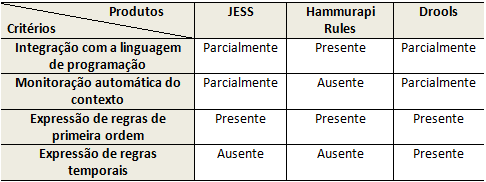
\includegraphics[angle=0,width=0.9\textwidth]{imagens//CompFerram.png}
%\end{table}

\begin{table}[ht]
\caption{Avaliação dos Motores de Inferência.} \label{tab:CompFerram}
\centering
\begin{tabular}{|l|l|l|l|}
\cline{2-4}
\multicolumn{1}{l|}{} & \multicolumn{3}{c|}{\textbf{Produtos}} \\ 
\hline
\textbf{Critérios} & \multicolumn{1}{c|}{\textbf{JESS}} & \multicolumn{1}{c|}{\textbf{Hummurapi} } & \multicolumn{1}{c|}{\textbf{Drools}} \\ 
 & \multicolumn{1}{c|}{} & \multicolumn{1}{c|}{\textbf{Rules}} & \multicolumn{1}{c|}{} \\ 
\hline
\multicolumn{1}{|c|}{\textbf{Integração com linguagem}} & \multicolumn{1}{c|}{Parcialmente} & \multicolumn{1}{c|}{Presente} & \multicolumn{1}{c|}{Parcialmente} \\ 
\multicolumn{1}{|c|}{\textbf{de programação}} & \multicolumn{1}{c|}{} & \multicolumn{1}{c|}{} & \multicolumn{1}{c|}{} \\ 
\hline
\multicolumn{1}{|c|}{\textbf{Monitoração automática do}} & \multicolumn{1}{c|}{Parcialmente} & \multicolumn{1}{c|}{Ausente} & \multicolumn{1}{c|}{Parcialmente} \\ 
\multicolumn{1}{|c|}{\textbf{contexto}} & \multicolumn{1}{c|}{} & \multicolumn{1}{c|}{} & \multicolumn{1}{c|}{} \\ 
\hline
\multicolumn{1}{|c|}{\textbf{Expressão de regras de}} & \multicolumn{1}{c|}{Presente} & \multicolumn{1}{c|}{Presente} & \multicolumn{1}{c|}{Presente} \\ 
\multicolumn{1}{|c|}{\textbf{primeira ordem}} & \multicolumn{1}{c|}{} & \multicolumn{1}{c|}{} & \multicolumn{1}{c|}{} \\ 
\hline
\multicolumn{1}{|c|}{\textbf{Expressão de regras}} & \multicolumn{1}{c|}{Ausente} & \multicolumn{1}{c|}{Ausente} & \multicolumn{1}{c|}{Presente} \\ 
\multicolumn{1}{|c|}{\textbf{temporais}} & \multicolumn{1}{c|}{} & \multicolumn{1}{c|}{} & \multicolumn{1}{c|}{} \\ 
\hline
\end{tabular}
\end{table}